\documentclass{standalone}
\usepackage{tikz}
\usetikzlibrary{
  arrows,
  calc,
  decorations.pathmorphing,
  decorations.pathreplacing,
  decorations.markings,
  fadings,
  positioning,
  shapes,
  arrows.meta
}
\usepgfmodule{oo}

\pgfdeclareradialshading{glow2}{\pgfpoint{0cm}{0cm}}{
  color(0mm)=(white);
  color(2mm)=(white);
  color(8mm)=(black);
  color(10mm)=(black)
}

\begin{tikzfadingfrompicture}[name=glow2 fading]
  \shade [shading=glow2] (0,0) circle (1);
\end{tikzfadingfrompicture}

\definecolor{atomblue}{rgb}{0,0,1}
\definecolor{atomorange}{rgb}{1,0.483,0}

\pgfdeclarelayer{tweezer}
\pgfsetlayers{tweezer,main}
\pgfooclass{tweezer}{
  \method tweezer() {
  }
  \method drawAtom(#1,#2,#3,#4) {
    \fill [#4,path fading=glow2 fading] (#1,#2) circle (#3);
  }
  \method drawNaAtom(#1,#2,#3) {
    \pgfoothis.drawAtom(#1,#2,#3,atomorange);
  }
  \method drawCsAtom(#1,#2,#3) {
    \pgfoothis.drawAtom(#1,#2,#3,blue);
  }
  \method drawMolecule(#1,#2,#3,#4){
    % x, y, len, angle
    \begin{scope}[shift={(#1, #2)}]
      \draw[line width=1] ({-#3 * cos(#4) / 2}, {-#3 * sin(#4) / 2})
      -- ({#3 * cos(#4) / 2}, {#3 * sin(#4) / 2});
      \begin{scope}[shift={({-#3 * cos(#4) / 2}, {-#3 * sin(#4) / 2})}]
        \pgfoothis.drawCsAtom(0, 0, 0.08);
      \end{scope}
      \begin{scope}[shift={({#3 * cos(#4) / 2}, {#3 * sin(#4) / 2})}]
        \pgfoothis.drawNaAtom(0, 0, 0.065);
      \end{scope}
    \end{scope}
  }
}
\pgfoonew \mytweezer=new tweezer()

\ifpdf
% Ensure reproducible output
\pdfinfoomitdate=1
\pdfsuppressptexinfo=-1
\pdftrailerid{}
\fi

\begin{document}

% Scale figure so that the text in the final plot is consistent with other figures
% note that the figure size needs to be scaled separately.
\begin{tikzpicture}[scale=1.27]
  \node at (0, 0) {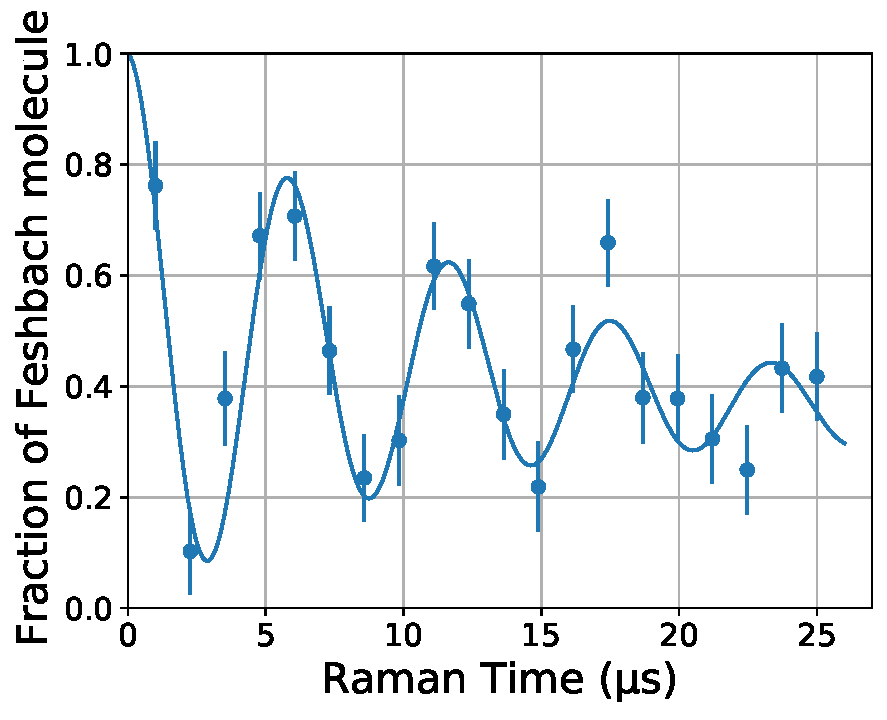
\includegraphics[width=6.75cm]{
      conclusion_ground_raman.pdf}};
  \mytweezer.drawMolecule(-1.65, 1.83, 0.22, 0)
  \mytweezer.drawMolecule(-0.95, 1.3, 0.22, 0)
  \mytweezer.drawMolecule(0.05, 0.9, 0.22, 0)

  \mytweezer.drawMolecule(-1.4, -1.25, 0.07, 0)
  \mytweezer.drawMolecule(-0.45, -0.88, 0.07, 0)
\end{tikzpicture}

\end{document}
